\documentclass[twoside]{book}

% Packages required by doxygen
\usepackage{fixltx2e}
\usepackage{calc}
\usepackage{doxygen}
\usepackage[export]{adjustbox} % also loads graphicx
\usepackage{graphicx}
\usepackage[utf8]{inputenc}
\usepackage{makeidx}
\usepackage{multicol}
\usepackage{multirow}
\PassOptionsToPackage{warn}{textcomp}
\usepackage{textcomp}
\usepackage[nointegrals]{wasysym}
\usepackage[table]{xcolor}

% Font selection
\usepackage[T1]{fontenc}
\usepackage[scaled=.90]{helvet}
\usepackage{courier}
\usepackage{amssymb}
\usepackage{sectsty}
\renewcommand{\familydefault}{\sfdefault}
\allsectionsfont{%
  \fontseries{bc}\selectfont%
  \color{darkgray}%
}
\renewcommand{\DoxyLabelFont}{%
  \fontseries{bc}\selectfont%
  \color{darkgray}%
}
\newcommand{\+}{\discretionary{\mbox{\scriptsize$\hookleftarrow$}}{}{}}

% Page & text layout
\usepackage{geometry}
\geometry{%
  a4paper,%
  top=2.5cm,%
  bottom=2.5cm,%
  left=2.5cm,%
  right=2.5cm%
}
\tolerance=750
\hfuzz=15pt
\hbadness=750
\setlength{\emergencystretch}{15pt}
\setlength{\parindent}{0cm}
\setlength{\parskip}{3ex plus 2ex minus 2ex}
\makeatletter
\renewcommand{\paragraph}{%
  \@startsection{paragraph}{4}{0ex}{-1.0ex}{1.0ex}{%
    \normalfont\normalsize\bfseries\SS@parafont%
  }%
}
\renewcommand{\subparagraph}{%
  \@startsection{subparagraph}{5}{0ex}{-1.0ex}{1.0ex}{%
    \normalfont\normalsize\bfseries\SS@subparafont%
  }%
}
\makeatother

% Headers & footers
\usepackage{fancyhdr}
\pagestyle{fancyplain}
\fancyhead[LE]{\fancyplain{}{\bfseries\thepage}}
\fancyhead[CE]{\fancyplain{}{}}
\fancyhead[RE]{\fancyplain{}{\bfseries\leftmark}}
\fancyhead[LO]{\fancyplain{}{\bfseries\rightmark}}
\fancyhead[CO]{\fancyplain{}{}}
\fancyhead[RO]{\fancyplain{}{\bfseries\thepage}}
\fancyfoot[LE]{\fancyplain{}{}}
\fancyfoot[CE]{\fancyplain{}{}}
\fancyfoot[RE]{\fancyplain{}{\bfseries\scriptsize Generated by Doxygen }}
\fancyfoot[LO]{\fancyplain{}{\bfseries\scriptsize Generated by Doxygen }}
\fancyfoot[CO]{\fancyplain{}{}}
\fancyfoot[RO]{\fancyplain{}{}}
\renewcommand{\footrulewidth}{0.4pt}
\renewcommand{\chaptermark}[1]{%
  \markboth{#1}{}%
}
\renewcommand{\sectionmark}[1]{%
  \markright{\thesection\ #1}%
}

% Indices & bibliography
\usepackage{natbib}
\usepackage[titles]{tocloft}
\setcounter{tocdepth}{3}
\setcounter{secnumdepth}{5}
\makeindex

% Hyperlinks (required, but should be loaded last)
\usepackage{ifpdf}
\ifpdf
  \usepackage[pdftex,pagebackref=true]{hyperref}
\else
  \usepackage[ps2pdf,pagebackref=true]{hyperref}
\fi
\hypersetup{%
  colorlinks=true,%
  linkcolor=blue,%
  citecolor=blue,%
  unicode%
}

% Custom commands
\newcommand{\clearemptydoublepage}{%
  \newpage{\pagestyle{empty}\cleardoublepage}%
}

\usepackage{caption}
\captionsetup{labelsep=space,justification=centering,font={bf},singlelinecheck=off,skip=4pt,position=top}

%===== C O N T E N T S =====

\begin{document}

% Titlepage & ToC
\hypersetup{pageanchor=false,
             bookmarksnumbered=true,
             pdfencoding=unicode
            }
\pagenumbering{alph}
\begin{titlepage}
\vspace*{7cm}
\begin{center}%
{\Large Spot\+Check }\\
\vspace*{1cm}
{\large Generated by Doxygen 1.8.13}\\
\end{center}
\end{titlepage}
\clearemptydoublepage
\pagenumbering{roman}
\tableofcontents
\clearemptydoublepage
\pagenumbering{arabic}
\hypersetup{pageanchor=true}

%--- Begin generated contents ---
\chapter{Deprecated List}
\label{deprecated}
\Hypertarget{deprecated}

\begin{DoxyRefList}
\item[\label{deprecated__deprecated000001}%
\Hypertarget{deprecated__deprecated000001}%
Member \hyperlink{classbackend_a63f2bdc2cb5376f087935230f6b7831d}{backend\+:\+:import\+\_\+source\+\_\+gal} (const callback\+\_\+info \&args)]The frontend now handles gal data imports. 
\end{DoxyRefList}
\chapter{Hierarchical Index}
\section{Class Hierarchy}
This inheritance list is sorted roughly, but not completely, alphabetically\+:\begin{DoxyCompactList}
\item \contentsline{section}{detail\+:\+:apply\+\_\+impl$<$ F, Tuple, Done, Total, N $>$}{\pageref{structdetail_1_1apply__impl}}{}
\item \contentsline{section}{detail\+:\+:apply\+\_\+impl$<$ F, Tuple, true, Total, N... $>$}{\pageref{structdetail_1_1apply__impl_3_01_f_00_01_tuple_00_01true_00_01_total_00_01_n_8_8_8_01_4}}{}
\item \contentsline{section}{async}{\pageref{structasync}}{}
\item Object\+Wrap\begin{DoxyCompactList}
\item \contentsline{section}{backend}{\pageref{classbackend}}{}
\end{DoxyCompactList}
\item \contentsline{section}{result}{\pageref{classresult}}{}
\item \contentsline{section}{backend\+:\+:Target}{\pageref{structbackend_1_1_target}}{}
\item \contentsline{section}{async\+:\+:work$<$ F, Args $>$}{\pageref{structasync_1_1work}}{}
\end{DoxyCompactList}

\chapter{Class Index}
\section{Class List}
Here are the classes, structs, unions and interfaces with brief descriptions\+:\begin{DoxyCompactList}
\item\contentsline{section}{\hyperlink{structdetail_1_1apply__impl}{detail\+::apply\+\_\+impl$<$ F, Tuple, Done, Total, N $>$} }{\pageref{structdetail_1_1apply__impl}}{}
\item\contentsline{section}{\hyperlink{structdetail_1_1apply__impl_3_01_f_00_01_tuple_00_01true_00_01_total_00_01_n_8_8_8_01_4}{detail\+::apply\+\_\+impl$<$ F, Tuple, true, Total, N... $>$} }{\pageref{structdetail_1_1apply__impl_3_01_f_00_01_tuple_00_01true_00_01_total_00_01_n_8_8_8_01_4}}{}
\item\contentsline{section}{\hyperlink{structasync}{async} }{\pageref{structasync}}{}
\item\contentsline{section}{\hyperlink{class_backend}{Backend} \\*The interface between Spotcheck\textquotesingle{}s analysis functions, Open\+CV, and the application\textquotesingle{}s frontend }{\pageref{class_backend}}{}
\item\contentsline{section}{\hyperlink{class_result}{Result} }{\pageref{class_result}}{}
\item\contentsline{section}{\hyperlink{struct_backend_1_1_target}{Backend\+::\+Target} }{\pageref{struct_backend_1_1_target}}{}
\item\contentsline{section}{\hyperlink{structasync_1_1work}{async\+::work$<$ F, Args $>$} }{\pageref{structasync_1_1work}}{}
\end{DoxyCompactList}

\chapter{File Index}
\section{File List}
Here is a list of all documented files with brief descriptions\+:\begin{DoxyCompactList}
\item\contentsline{section}{\hyperlink{analysis_8hpp}{analysis.\+hpp} \\*Analysis Functions }{\pageref{analysis_8hpp}}{}
\item\contentsline{section}{{\bfseries async.\+hpp} }{\pageref{async_8hpp}}{}
\item\contentsline{section}{\hyperlink{backend_8hpp}{backend.\+hpp} \\*Backend Module }{\pageref{backend_8hpp}}{}
\item\contentsline{section}{{\bfseries make\+\_\+cv\+\_\+roi.\+hpp} }{\pageref{make__cv__roi_8hpp}}{}
\item\contentsline{section}{{\bfseries preview\+\_\+normalized.\+hpp} }{\pageref{preview__normalized_8hpp}}{}
\item\contentsline{section}{{\bfseries results.\+hpp} }{\pageref{results_8hpp}}{}
\end{DoxyCompactList}

\chapter{Class Documentation}
\hypertarget{structdetail_1_1apply__impl}{}\section{detail\+:\+:apply\+\_\+impl$<$ F, Tuple, Done, Total, N $>$ Struct Template Reference}
\label{structdetail_1_1apply__impl}\index{detail\+::apply\+\_\+impl$<$ F, Tuple, Done, Total, N $>$@{detail\+::apply\+\_\+impl$<$ F, Tuple, Done, Total, N $>$}}
\subsection*{Static Public Member Functions}
\begin{DoxyCompactItemize}
\item 
\mbox{\Hypertarget{structdetail_1_1apply__impl_aeb8ceae999d656f153245ec45b5c7c6c}\label{structdetail_1_1apply__impl_aeb8ceae999d656f153245ec45b5c7c6c}} 
static void {\bfseries apply} (F f, Tuple \&\&t)
\end{DoxyCompactItemize}


The documentation for this struct was generated from the following file\+:\begin{DoxyCompactItemize}
\item 
async.\+hpp\end{DoxyCompactItemize}

\hypertarget{structdetail_1_1apply__impl_3_01_f_00_01_tuple_00_01true_00_01_total_00_01_n_8_8_8_01_4}{}\section{detail\+:\+:apply\+\_\+impl$<$ F, Tuple, true, Total, N... $>$ Struct Template Reference}
\label{structdetail_1_1apply__impl_3_01_f_00_01_tuple_00_01true_00_01_total_00_01_n_8_8_8_01_4}\index{detail\+::apply\+\_\+impl$<$ F, Tuple, true, Total, N... $>$@{detail\+::apply\+\_\+impl$<$ F, Tuple, true, Total, N... $>$}}
\subsection*{Static Public Member Functions}
\begin{DoxyCompactItemize}
\item 
\mbox{\Hypertarget{structdetail_1_1apply__impl_3_01_f_00_01_tuple_00_01true_00_01_total_00_01_n_8_8_8_01_4_a66cf9d7c78c88f55ee6f435a4fa600da}\label{structdetail_1_1apply__impl_3_01_f_00_01_tuple_00_01true_00_01_total_00_01_n_8_8_8_01_4_a66cf9d7c78c88f55ee6f435a4fa600da}} 
static void {\bfseries apply} (F f, Tuple \&\&t)
\end{DoxyCompactItemize}


The documentation for this struct was generated from the following file\+:\begin{DoxyCompactItemize}
\item 
async.\+hpp\end{DoxyCompactItemize}

\hypertarget{structasync}{}\section{async Struct Reference}
\label{structasync}\index{async@{async}}
\subsection*{Classes}
\begin{DoxyCompactItemize}
\item 
struct \hyperlink{structasync_1_1work}{work}
\end{DoxyCompactItemize}
\subsection*{Static Public Member Functions}
\begin{DoxyCompactItemize}
\item 
\mbox{\Hypertarget{structasync_a888d644635083c1d3bf8eb160c3935ac}\label{structasync_a888d644635083c1d3bf8eb160c3935ac}} 
{\footnotesize template$<$typename F , typename... Args$>$ }\\static void {\bfseries start} (const js\+\_\+cb \&callback, F \&\&work\+\_\+routine, Args \&\&... args)
\end{DoxyCompactItemize}


The documentation for this struct was generated from the following file\+:\begin{DoxyCompactItemize}
\item 
async.\+hpp\end{DoxyCompactItemize}

\hypertarget{classbackend}{}\section{backend Class Reference}
\label{classbackend}\index{backend@{backend}}
Inheritance diagram for backend\+:\begin{figure}[H]
\begin{center}
\leavevmode
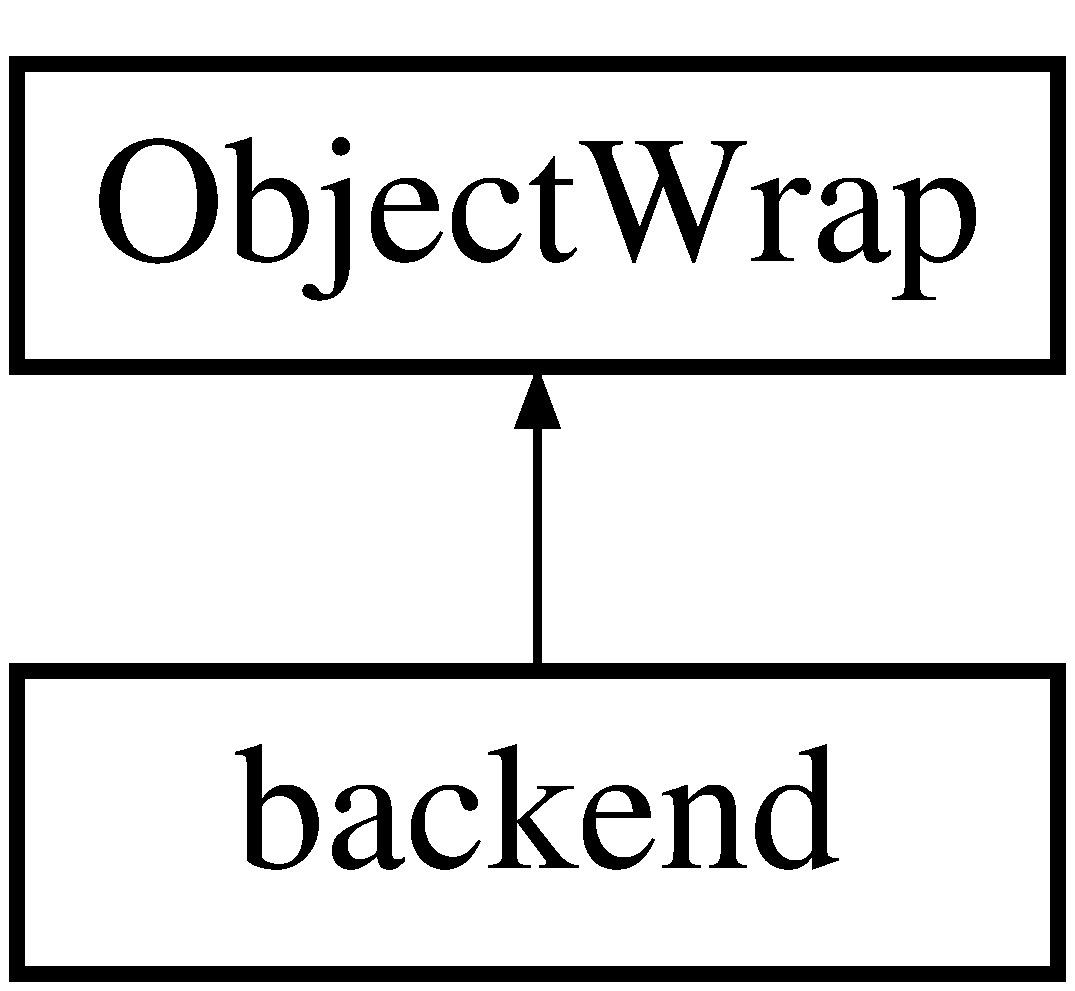
\includegraphics[height=2.000000cm]{classbackend}
\end{center}
\end{figure}
\subsection*{Classes}
\begin{DoxyCompactItemize}
\item 
struct \hyperlink{structbackend_1_1_target}{Target}
\end{DoxyCompactItemize}
\subsection*{Public Types}
\begin{DoxyCompactItemize}
\item 
\mbox{\Hypertarget{classbackend_aa165cfc3da158f073832ef1f6ce4e1b8}\label{classbackend_aa165cfc3da158f073832ef1f6ce4e1b8}} 
using {\bfseries callback\+\_\+info} = v8\+::\+Function\+Callback\+Info$<$ v8\+::\+Value $>$
\end{DoxyCompactItemize}
\subsection*{Static Public Member Functions}
\begin{DoxyCompactItemize}
\item 
static void \hyperlink{classbackend_a44ff4b919d81243742ff4b4bedde4f83}{init} (v8\+::\+Local$<$ v8\+::\+Object $>$ exports, v8\+::\+Local$<$ v8\+::\+Object $>$ module)
\begin{DoxyCompactList}\small\item\em Initializes the backend module. \end{DoxyCompactList}\item 
static void \hyperlink{classbackend_a9e8157df648d308880c4ec62adc426fb}{alloc} (const callback\+\_\+info \&args)
\begin{DoxyCompactList}\small\item\em Allocates a new backend object. \end{DoxyCompactList}\item 
static void \hyperlink{classbackend_a516007959f2bc8b4f5f83d1a448a6090}{import\+\_\+source\+\_\+image} (const callback\+\_\+info \&args)
\begin{DoxyCompactList}\small\item\em Imports the source image into the backend. \end{DoxyCompactList}\item 
static void \hyperlink{classbackend_a63f2bdc2cb5376f087935230f6b7831d}{import\+\_\+source\+\_\+gal} (const callback\+\_\+info \&args)
\begin{DoxyCompactList}\small\item\em Imports the source gal into the backend. \end{DoxyCompactList}\item 
static void \hyperlink{classbackend_a3b212ebed9184a5818c9ce81b5513a3c}{split\+\_\+sectors} (const callback\+\_\+info \&args)
\begin{DoxyCompactList}\small\item\em Splits the backend\textquotesingle{}s heightmap into smaller chunks. \end{DoxyCompactList}\item 
static void \hyperlink{classbackend_a3831c36d689d4a5dfa696902c6cac0d1}{clear\+\_\+targets} (const callback\+\_\+info \&args)
\begin{DoxyCompactList}\small\item\em Clears the backend\textquotesingle{}s analysis targets. \end{DoxyCompactList}\item 
static void \hyperlink{classbackend_adea4e670e5c1e84d295c5cd03deceb4a}{launch\+\_\+analysis} (const callback\+\_\+info \&args)
\begin{DoxyCompactList}\small\item\em Launches analysis on all of the backend\textquotesingle{}s analysis targets. \end{DoxyCompactList}\item 
static void \hyperlink{classbackend_a23963a7c7e73bba71cbf77e27224efd8}{analyze\+\_\+target} (\hyperlink{structbackend_1_1_target}{Target} \&target, cv\+::\+Mat \&src, cv\+::\+Mat \&mask)
\begin{DoxyCompactList}\small\item\em Runs analysis on a single analysis target. \end{DoxyCompactList}\item 
static void \hyperlink{classbackend_ac981fabc3077c133dca35b5cb7e6f66c}{add\+\_\+target} (const callback\+\_\+info \&args)
\begin{DoxyCompactList}\small\item\em Adds an analysis target to the backend. \end{DoxyCompactList}\item 
static void \hyperlink{classbackend_a827177f07a64774f20057d1704e43a5b}{get\+\_\+target\+\_\+thresh} (const callback\+\_\+info \&args)
\begin{DoxyCompactList}\small\item\em Gets the threshold value for a target. \end{DoxyCompactList}\item 
static void \hyperlink{classbackend_a91fe1ff0bbdc9e29d6958e0cf72d10ba}{write\+\_\+results\+\_\+\+J\+S\+ON} (const callback\+\_\+info \&args)
\begin{DoxyCompactList}\small\item\em Serialize the backend\textquotesingle{}s results to a J\+S\+ON format. \end{DoxyCompactList}\item 
static void \hyperlink{classbackend_a567b1f81aaa959b25ab5448752a5a371}{update\+\_\+target\+\_\+thresh} (const callback\+\_\+info \&args)
\begin{DoxyCompactList}\small\item\em Updates the threshold value for an analysis target. \end{DoxyCompactList}\item 
static void \hyperlink{classbackend_aa4a237c847f3bdc527b7bf01f2fa1974}{provide\+\_\+norm\+\_\+preview} (const callback\+\_\+info \&args)
\begin{DoxyCompactList}\small\item\em Provides a preview of the entire heighmap. \end{DoxyCompactList}\item 
static void \hyperlink{classbackend_aea5762a8de17d93aadb8d1a870e1474d}{is\+\_\+busy} (const callback\+\_\+info \&args)
\begin{DoxyCompactList}\small\item\em Queries whether the backend is working on analysis targets. \end{DoxyCompactList}\end{DoxyCompactItemize}
\subsection*{Static Public Attributes}
\begin{DoxyCompactItemize}
\item 
\mbox{\Hypertarget{classbackend_a2e36e089be85fa5fcdec6d9ab50c3199}\label{classbackend_a2e36e089be85fa5fcdec6d9ab50c3199}} 
static v8\+::\+Persistent$<$ v8\+::\+Function $>$ {\bfseries constructor}
\end{DoxyCompactItemize}


\subsection{Member Function Documentation}
\mbox{\Hypertarget{classbackend_ac981fabc3077c133dca35b5cb7e6f66c}\label{classbackend_ac981fabc3077c133dca35b5cb7e6f66c}} 
\index{backend@{backend}!add\+\_\+target@{add\+\_\+target}}
\index{add\+\_\+target@{add\+\_\+target}!backend@{backend}}
\subsubsection{\texorpdfstring{add\+\_\+target()}{add\_target()}}
{\footnotesize\ttfamily void backend\+::add\+\_\+target (\begin{DoxyParamCaption}\item[{const callback\+\_\+info \&}]{args }\end{DoxyParamCaption})\hspace{0.3cm}{\ttfamily [static]}}



Adds an analysis target to the backend. 

This function is part of the backend javascript A\+PI. It adds an analysis target to the backend, where each target is metadata that describes the subregion of the image to be analysed. From javascript, it takes seven parameters\+: 1) row\+Id\+: The row of the selection grid where the subimage lies. 2) col\+Id\+: The column of the selection grid where the subimage lies. 3) fract\+Startx\+: The x percentage into the image where the subimage begins. 4) fract\+Starty\+: The y percentage into the image where the subimage begins. 5) fract\+Endx\+: The x percentage into the image where the subimage ends. 6) fract\+Endy\+: The y percentage into the image where the subimage ends. 7) threshold\+: A default threshold value (unused) \mbox{\Hypertarget{classbackend_a9e8157df648d308880c4ec62adc426fb}\label{classbackend_a9e8157df648d308880c4ec62adc426fb}} 
\index{backend@{backend}!alloc@{alloc}}
\index{alloc@{alloc}!backend@{backend}}
\subsubsection{\texorpdfstring{alloc()}{alloc()}}
{\footnotesize\ttfamily void backend\+::alloc (\begin{DoxyParamCaption}\item[{const callback\+\_\+info \&}]{args }\end{DoxyParamCaption})\hspace{0.3cm}{\ttfamily [static]}}



Allocates a new backend object. 

This function is part of the backend javascript A\+PI. It is called upon allocation of a new backend object by the frontend, and is responsible for performing the initial memory allocation.

\begin{DoxyReturn}{Returns}
A backend javascript object. 
\end{DoxyReturn}
\mbox{\Hypertarget{classbackend_a23963a7c7e73bba71cbf77e27224efd8}\label{classbackend_a23963a7c7e73bba71cbf77e27224efd8}} 
\index{backend@{backend}!analyze\+\_\+target@{analyze\+\_\+target}}
\index{analyze\+\_\+target@{analyze\+\_\+target}!backend@{backend}}
\subsubsection{\texorpdfstring{analyze\+\_\+target()}{analyze\_target()}}
{\footnotesize\ttfamily void backend\+::analyze\+\_\+target (\begin{DoxyParamCaption}\item[{\hyperlink{structbackend_1_1_target}{Target} \&}]{target,  }\item[{cv\+::\+Mat \&}]{src,  }\item[{cv\+::\+Mat \&}]{mask }\end{DoxyParamCaption})\hspace{0.3cm}{\ttfamily [static]}}



Runs analysis on a single analysis target. 

This function runs the full suite of analysis metrics on a subregion of the heightmap. Upon completion, it writes a result object to the backend\textquotesingle{}s list of results.


\begin{DoxyParams}{Parameters}
{\em target} & The target struct with metadata about the target subregion \\
\hline
{\em src} & The original source image representing the subregion \\
\hline
{\em mask} & A binary mask of the subregion representing droplet location \\
\hline
\end{DoxyParams}
\mbox{\Hypertarget{classbackend_a3831c36d689d4a5dfa696902c6cac0d1}\label{classbackend_a3831c36d689d4a5dfa696902c6cac0d1}} 
\index{backend@{backend}!clear\+\_\+targets@{clear\+\_\+targets}}
\index{clear\+\_\+targets@{clear\+\_\+targets}!backend@{backend}}
\subsubsection{\texorpdfstring{clear\+\_\+targets()}{clear\_targets()}}
{\footnotesize\ttfamily void backend\+::clear\+\_\+targets (\begin{DoxyParamCaption}\item[{const callback\+\_\+info \&}]{args }\end{DoxyParamCaption})\hspace{0.3cm}{\ttfamily [static]}}



Clears the backend\textquotesingle{}s analysis targets. 

This function is part of the backend javascript A\+PI. It clears out the list of analysis targets maintained by the backend. \mbox{\Hypertarget{classbackend_a827177f07a64774f20057d1704e43a5b}\label{classbackend_a827177f07a64774f20057d1704e43a5b}} 
\index{backend@{backend}!get\+\_\+target\+\_\+thresh@{get\+\_\+target\+\_\+thresh}}
\index{get\+\_\+target\+\_\+thresh@{get\+\_\+target\+\_\+thresh}!backend@{backend}}
\subsubsection{\texorpdfstring{get\+\_\+target\+\_\+thresh()}{get\_target\_thresh()}}
{\footnotesize\ttfamily void backend\+::get\+\_\+target\+\_\+thresh (\begin{DoxyParamCaption}\item[{const callback\+\_\+info \&}]{args }\end{DoxyParamCaption})\hspace{0.3cm}{\ttfamily [static]}}



Gets the threshold value for a target. 

This function is part of the backend javascript A\+PI. It takes two parameters, the target row followed by the target column of the desired subimage to the current threshold value for. \mbox{\Hypertarget{classbackend_a63f2bdc2cb5376f087935230f6b7831d}\label{classbackend_a63f2bdc2cb5376f087935230f6b7831d}} 
\index{backend@{backend}!import\+\_\+source\+\_\+gal@{import\+\_\+source\+\_\+gal}}
\index{import\+\_\+source\+\_\+gal@{import\+\_\+source\+\_\+gal}!backend@{backend}}
\subsubsection{\texorpdfstring{import\+\_\+source\+\_\+gal()}{import\_source\_gal()}}
{\footnotesize\ttfamily void backend\+::import\+\_\+source\+\_\+gal (\begin{DoxyParamCaption}\item[{const callback\+\_\+info \&}]{args }\end{DoxyParamCaption})\hspace{0.3cm}{\ttfamily [static]}}



Imports the source gal into the backend. 

This function is part of the backend javascript A\+PI. It takes two javascript objects as parameters; a path to the gal file to be loaded and a callback to execute upon completion.

\begin{DoxyRefDesc}{Deprecated}
\item[\hyperlink{deprecated__deprecated000001}{Deprecated}]The frontend now handles gal data imports. \end{DoxyRefDesc}
\mbox{\Hypertarget{classbackend_a516007959f2bc8b4f5f83d1a448a6090}\label{classbackend_a516007959f2bc8b4f5f83d1a448a6090}} 
\index{backend@{backend}!import\+\_\+source\+\_\+image@{import\+\_\+source\+\_\+image}}
\index{import\+\_\+source\+\_\+image@{import\+\_\+source\+\_\+image}!backend@{backend}}
\subsubsection{\texorpdfstring{import\+\_\+source\+\_\+image()}{import\_source\_image()}}
{\footnotesize\ttfamily void backend\+::import\+\_\+source\+\_\+image (\begin{DoxyParamCaption}\item[{const callback\+\_\+info \&}]{args }\end{DoxyParamCaption})\hspace{0.3cm}{\ttfamily [static]}}



Imports the source image into the backend. 

This function is part of the backend javascript A\+PI. It takes two javascript objects as parameters; a path to the image to be loaded and a callback to execute upon completion. \mbox{\Hypertarget{classbackend_a44ff4b919d81243742ff4b4bedde4f83}\label{classbackend_a44ff4b919d81243742ff4b4bedde4f83}} 
\index{backend@{backend}!init@{init}}
\index{init@{init}!backend@{backend}}
\subsubsection{\texorpdfstring{init()}{init()}}
{\footnotesize\ttfamily void backend\+::init (\begin{DoxyParamCaption}\item[{v8\+::\+Local$<$ v8\+::\+Object $>$}]{exports,  }\item[{v8\+::\+Local$<$ v8\+::\+Object $>$}]{module }\end{DoxyParamCaption})\hspace{0.3cm}{\ttfamily [static]}}



Initializes the backend module. 

This function is part of the backend javascript A\+PI. It is responsible for performing the mapping between this class\textquotesingle{} static members and the javascript A\+PI functions accessible from the frontend. \mbox{\Hypertarget{classbackend_aea5762a8de17d93aadb8d1a870e1474d}\label{classbackend_aea5762a8de17d93aadb8d1a870e1474d}} 
\index{backend@{backend}!is\+\_\+busy@{is\+\_\+busy}}
\index{is\+\_\+busy@{is\+\_\+busy}!backend@{backend}}
\subsubsection{\texorpdfstring{is\+\_\+busy()}{is\_busy()}}
{\footnotesize\ttfamily void backend\+::is\+\_\+busy (\begin{DoxyParamCaption}\item[{const callback\+\_\+info \&}]{args }\end{DoxyParamCaption})\hspace{0.3cm}{\ttfamily [static]}}



Queries whether the backend is working on analysis targets. 

This function is part of the backend javascript A\+PI. It returns true if the backend has no more analysis tasks to complete. \mbox{\Hypertarget{classbackend_adea4e670e5c1e84d295c5cd03deceb4a}\label{classbackend_adea4e670e5c1e84d295c5cd03deceb4a}} 
\index{backend@{backend}!launch\+\_\+analysis@{launch\+\_\+analysis}}
\index{launch\+\_\+analysis@{launch\+\_\+analysis}!backend@{backend}}
\subsubsection{\texorpdfstring{launch\+\_\+analysis()}{launch\_analysis()}}
{\footnotesize\ttfamily void backend\+::launch\+\_\+analysis (\begin{DoxyParamCaption}\item[{const callback\+\_\+info \&}]{args }\end{DoxyParamCaption})\hspace{0.3cm}{\ttfamily [static]}}



Launches analysis on all of the backend\textquotesingle{}s analysis targets. 

This function is part of the backend javascript A\+PI. It launches an analysis run, which submits an asynchronous task for each analysis target, each of which calls \hyperlink{classbackend_a23963a7c7e73bba71cbf77e27224efd8}{backend\+::analyze\+\_\+target} on the dataset for that target. \mbox{\Hypertarget{classbackend_aa4a237c847f3bdc527b7bf01f2fa1974}\label{classbackend_aa4a237c847f3bdc527b7bf01f2fa1974}} 
\index{backend@{backend}!provide\+\_\+norm\+\_\+preview@{provide\+\_\+norm\+\_\+preview}}
\index{provide\+\_\+norm\+\_\+preview@{provide\+\_\+norm\+\_\+preview}!backend@{backend}}
\subsubsection{\texorpdfstring{provide\+\_\+norm\+\_\+preview()}{provide\_norm\_preview()}}
{\footnotesize\ttfamily void backend\+::provide\+\_\+norm\+\_\+preview (\begin{DoxyParamCaption}\item[{const callback\+\_\+info \&}]{args }\end{DoxyParamCaption})\hspace{0.3cm}{\ttfamily [static]}}



Provides a preview of the entire heighmap. 

This function is part of the backend javascript A\+PI. It takes one parameter, a callback to be executed upon completion. \mbox{\Hypertarget{classbackend_a3b212ebed9184a5818c9ce81b5513a3c}\label{classbackend_a3b212ebed9184a5818c9ce81b5513a3c}} 
\index{backend@{backend}!split\+\_\+sectors@{split\+\_\+sectors}}
\index{split\+\_\+sectors@{split\+\_\+sectors}!backend@{backend}}
\subsubsection{\texorpdfstring{split\+\_\+sectors()}{split\_sectors()}}
{\footnotesize\ttfamily void backend\+::split\+\_\+sectors (\begin{DoxyParamCaption}\item[{const callback\+\_\+info \&}]{args }\end{DoxyParamCaption})\hspace{0.3cm}{\ttfamily [static]}}



Splits the backend\textquotesingle{}s heightmap into smaller chunks. 

This function is part of the backend javascript A\+PI. It splits the source heightmap into smaller subimages based on the list of targets previously specified by calling \hyperlink{classbackend_ac981fabc3077c133dca35b5cb7e6f66c}{backend.\+add\+\_\+target}(...). After processing each sector, it writes three images to the directory frontend/temp/\+: the original segmented image, a binary mask representing where the microarray droplet might be located within the image, and a normalized image for easier viewing within the frontend. \mbox{\Hypertarget{classbackend_a567b1f81aaa959b25ab5448752a5a371}\label{classbackend_a567b1f81aaa959b25ab5448752a5a371}} 
\index{backend@{backend}!update\+\_\+target\+\_\+thresh@{update\+\_\+target\+\_\+thresh}}
\index{update\+\_\+target\+\_\+thresh@{update\+\_\+target\+\_\+thresh}!backend@{backend}}
\subsubsection{\texorpdfstring{update\+\_\+target\+\_\+thresh()}{update\_target\_thresh()}}
{\footnotesize\ttfamily void backend\+::update\+\_\+target\+\_\+thresh (\begin{DoxyParamCaption}\item[{const callback\+\_\+info \&}]{args }\end{DoxyParamCaption})\hspace{0.3cm}{\ttfamily [static]}}



Updates the threshold value for an analysis target. 

This function is part of the backend javascript A\+PI. It takes four parameters; a callback, followed by the row and column describing which target to modify, then the substitute threshold value. \mbox{\Hypertarget{classbackend_a91fe1ff0bbdc9e29d6958e0cf72d10ba}\label{classbackend_a91fe1ff0bbdc9e29d6958e0cf72d10ba}} 
\index{backend@{backend}!write\+\_\+results\+\_\+\+J\+S\+ON@{write\+\_\+results\+\_\+\+J\+S\+ON}}
\index{write\+\_\+results\+\_\+\+J\+S\+ON@{write\+\_\+results\+\_\+\+J\+S\+ON}!backend@{backend}}
\subsubsection{\texorpdfstring{write\+\_\+results\+\_\+\+J\+S\+O\+N()}{write\_results\_JSON()}}
{\footnotesize\ttfamily void backend\+::write\+\_\+results\+\_\+\+J\+S\+ON (\begin{DoxyParamCaption}\item[{const callback\+\_\+info \&}]{args }\end{DoxyParamCaption})\hspace{0.3cm}{\ttfamily [static]}}



Serialize the backend\textquotesingle{}s results to a J\+S\+ON format. 

This function is part of the backend javascript A\+PI. It takes one parameter, a javascript callback function to be called when serialization finishes. The backend writes results to the path frontend/temp/results.\+json. 

The documentation for this class was generated from the following files\+:\begin{DoxyCompactItemize}
\item 
\hyperlink{backend_8hpp}{backend.\+hpp}\item 
backend.\+cpp\end{DoxyCompactItemize}

\hypertarget{classresult}{}\section{result Class Reference}
\label{classresult}\index{result@{result}}


The documentation for this class was generated from the following file\+:\begin{DoxyCompactItemize}
\item 
\hyperlink{results_8hpp}{results.\+hpp}\end{DoxyCompactItemize}

\hypertarget{structbackend_1_1_target}{}\section{backend\+:\+:Target Struct Reference}
\label{structbackend_1_1_target}\index{backend\+::\+Target@{backend\+::\+Target}}
\subsection*{Public Attributes}
\begin{DoxyCompactItemize}
\item 
\mbox{\Hypertarget{structbackend_1_1_target_a82a3cc2354c8f5cc8f73dd035686a7ae}\label{structbackend_1_1_target_a82a3cc2354c8f5cc8f73dd035686a7ae}} 
int64\+\_\+t {\bfseries row\+Id}
\item 
\mbox{\Hypertarget{structbackend_1_1_target_adb150295c006beca37c931d0a9d075e5}\label{structbackend_1_1_target_adb150295c006beca37c931d0a9d075e5}} 
int64\+\_\+t {\bfseries col\+Id}
\item 
\mbox{\Hypertarget{structbackend_1_1_target_ace53ce7fb79199d53843ba786dd7d8ee}\label{structbackend_1_1_target_ace53ce7fb79199d53843ba786dd7d8ee}} 
double {\bfseries fract\+Startx}
\item 
\mbox{\Hypertarget{structbackend_1_1_target_a7c0c2652d93975e915e4b6b038116bce}\label{structbackend_1_1_target_a7c0c2652d93975e915e4b6b038116bce}} 
double {\bfseries fract\+Starty}
\item 
\mbox{\Hypertarget{structbackend_1_1_target_ace16e945fc4900abf2a809abd24387ae}\label{structbackend_1_1_target_ace16e945fc4900abf2a809abd24387ae}} 
double {\bfseries fract\+Endx}
\item 
\mbox{\Hypertarget{structbackend_1_1_target_a8a607576d003f341eec9bcdefc5abde8}\label{structbackend_1_1_target_a8a607576d003f341eec9bcdefc5abde8}} 
double {\bfseries fract\+Endy}
\item 
\mbox{\Hypertarget{structbackend_1_1_target_a89d5a494c6baf04c5d64443d9c7bf3f6}\label{structbackend_1_1_target_a89d5a494c6baf04c5d64443d9c7bf3f6}} 
int64\+\_\+t {\bfseries threshold}
\end{DoxyCompactItemize}


The documentation for this struct was generated from the following file\+:\begin{DoxyCompactItemize}
\item 
backend.\+hpp\end{DoxyCompactItemize}

\hypertarget{structasync_1_1work}{}\section{async\+:\+:work$<$ F, Args $>$ Struct Template Reference}
\label{structasync_1_1work}\index{async\+::work$<$ F, Args $>$@{async\+::work$<$ F, Args $>$}}
\subsection*{Public Member Functions}
\begin{DoxyCompactItemize}
\item 
\mbox{\Hypertarget{structasync_1_1work_a95ae3bc60696f23f55113ee489bdfbf0}\label{structasync_1_1work_a95ae3bc60696f23f55113ee489bdfbf0}} 
{\bfseries work} (F \&\&work\+\_\+routine, Args \&\&... args)
\end{DoxyCompactItemize}
\subsection*{Public Attributes}
\begin{DoxyCompactItemize}
\item 
\mbox{\Hypertarget{structasync_1_1work_a718407ebe74d4d16540444560b44727d}\label{structasync_1_1work_a718407ebe74d4d16540444560b44727d}} 
uv\+\_\+work\+\_\+t {\bfseries m\+\_\+request}
\item 
\mbox{\Hypertarget{structasync_1_1work_af18ee6164b7b2a244e746d8405ed8c02}\label{structasync_1_1work_af18ee6164b7b2a244e746d8405ed8c02}} 
js\+\_\+persist\+\_\+cb {\bfseries m\+\_\+callback}
\item 
\mbox{\Hypertarget{structasync_1_1work_a1b466f9efcce8d24660720f11f759a61}\label{structasync_1_1work_a1b466f9efcce8d24660720f11f759a61}} 
F {\bfseries m\+\_\+work\+\_\+routine}
\item 
\mbox{\Hypertarget{structasync_1_1work_a7881da189c74cfc6458831277cb71205}\label{structasync_1_1work_a7881da189c74cfc6458831277cb71205}} 
std\+::tuple$<$ Args... $>$ {\bfseries m\+\_\+work\+\_\+args}
\end{DoxyCompactItemize}


The documentation for this struct was generated from the following file\+:\begin{DoxyCompactItemize}
\item 
async.\+hpp\end{DoxyCompactItemize}

\chapter{File Documentation}
\hypertarget{analysis_8hpp}{}\section{analysis.\+hpp File Reference}
\label{analysis_8hpp}\index{analysis.\+hpp@{analysis.\+hpp}}


Analysis Functions.  


{\ttfamily \#include $<$opencv2/imgproc/imgproc.\+hpp$>$}\newline
{\ttfamily \#include $<$iostream$>$}\newline
{\ttfamily \#include $<$opencv2/highgui/highgui.\+hpp$>$}\newline
{\ttfamily \#include $<$stdio.\+h$>$}\newline
{\ttfamily \#include $<$stdlib.\+h$>$}\newline
{\ttfamily \#include $<$algorithm$>$}\newline
\subsection*{Functions}
\begin{DoxyCompactItemize}
\item 
int \hyperlink{analysis_8hpp_a9e252dfc1a70e6524a3b74d23d8d8092}{find\+\_\+background} (cv\+::\+Mat \&src, cv\+::\+Mat \&mask)
\begin{DoxyCompactList}\small\item\em Calculates a target\textquotesingle{}s the average background value. \end{DoxyCompactList}\item 
int \hyperlink{analysis_8hpp_a068116eb59ea8433c8c9cc020a15fb2e}{find\+\_\+area} (cv\+::\+Mat \&src, cv\+::\+Mat \&mask)
\begin{DoxyCompactList}\small\item\em Calculates a target\textquotesingle{}s area. \end{DoxyCompactList}\item 
unsigned char \hyperlink{analysis_8hpp_a3dc19d7b5aa9e517a3ccfef69d66b764}{find\+\_\+max\+\_\+height} (cv\+::\+Mat \&src, cv\+::\+Mat \&mask, int bg\+Height)
\item 
unsigned char \hyperlink{analysis_8hpp_a05d683bfb77875967d79ad5fdfa79a2c}{find\+\_\+min\+\_\+height} (cv\+::\+Mat \&src, cv\+::\+Mat \&mask, int bg\+Height)
\item 
long \hyperlink{analysis_8hpp_a293679f9c37eef65c42a1d2bd228e8e5}{find\+\_\+volume} (cv\+::\+Mat \&src, cv\+::\+Mat \&mask, int bg\+Height)
\begin{DoxyCompactList}\small\item\em Calculates a target\textquotesingle{}s volume. \end{DoxyCompactList}\item 
long \hyperlink{analysis_8hpp_aa0a3d6be0b6848039ec16fb288641b35}{find\+\_\+average\+\_\+height} (cv\+::\+Mat \&src, cv\+::\+Mat \&mask, int bg\+Height)
\begin{DoxyCompactList}\small\item\em Calculates a target\textquotesingle{}s average height. \end{DoxyCompactList}\item 
\mbox{\Hypertarget{analysis_8hpp_adb1b33ece4dfa48222af9f0d5d6bba71}\label{analysis_8hpp_adb1b33ece4dfa48222af9f0d5d6bba71}} 
double {\bfseries find\+\_\+circularity} (cv\+::\+Mat \&mask)
\end{DoxyCompactItemize}


\subsection{Detailed Description}
Analysis Functions. 



\subsection{Function Documentation}
\mbox{\Hypertarget{analysis_8hpp_a068116eb59ea8433c8c9cc020a15fb2e}\label{analysis_8hpp_a068116eb59ea8433c8c9cc020a15fb2e}} 
\index{analysis.\+hpp@{analysis.\+hpp}!find\+\_\+area@{find\+\_\+area}}
\index{find\+\_\+area@{find\+\_\+area}!analysis.\+hpp@{analysis.\+hpp}}
\subsubsection{\texorpdfstring{find\+\_\+area()}{find\_area()}}
{\footnotesize\ttfamily int find\+\_\+area (\begin{DoxyParamCaption}\item[{cv\+::\+Mat \&}]{src,  }\item[{cv\+::\+Mat \&}]{mask }\end{DoxyParamCaption})}



Calculates a target\textquotesingle{}s area. 

This function calulates a target\textquotesingle{}s area by computing an integral of all of the binary mask\textquotesingle{}s nonzero pixels.


\begin{DoxyParams}{Parameters}
{\em src} & The heightmap source subimage \\
\hline
{\em mask} & The binary droplet dection mask \\
\hline
\end{DoxyParams}
\mbox{\Hypertarget{analysis_8hpp_aa0a3d6be0b6848039ec16fb288641b35}\label{analysis_8hpp_aa0a3d6be0b6848039ec16fb288641b35}} 
\index{analysis.\+hpp@{analysis.\+hpp}!find\+\_\+average\+\_\+height@{find\+\_\+average\+\_\+height}}
\index{find\+\_\+average\+\_\+height@{find\+\_\+average\+\_\+height}!analysis.\+hpp@{analysis.\+hpp}}
\subsubsection{\texorpdfstring{find\+\_\+average\+\_\+height()}{find\_average\_height()}}
{\footnotesize\ttfamily long find\+\_\+average\+\_\+height (\begin{DoxyParamCaption}\item[{cv\+::\+Mat \&}]{src,  }\item[{cv\+::\+Mat \&}]{mask,  }\item[{int}]{bg\+Height }\end{DoxyParamCaption})}



Calculates a target\textquotesingle{}s average height. 

This function works calculates the average height of a target.


\begin{DoxyParams}{Parameters}
{\em src} & The heightmap source subimage \\
\hline
{\em mask} & The binary droplet dection mask \\
\hline
\end{DoxyParams}
\mbox{\Hypertarget{analysis_8hpp_a9e252dfc1a70e6524a3b74d23d8d8092}\label{analysis_8hpp_a9e252dfc1a70e6524a3b74d23d8d8092}} 
\index{analysis.\+hpp@{analysis.\+hpp}!find\+\_\+background@{find\+\_\+background}}
\index{find\+\_\+background@{find\+\_\+background}!analysis.\+hpp@{analysis.\+hpp}}
\subsubsection{\texorpdfstring{find\+\_\+background()}{find\_background()}}
{\footnotesize\ttfamily int find\+\_\+background (\begin{DoxyParamCaption}\item[{cv\+::\+Mat \&}]{src,  }\item[{cv\+::\+Mat \&}]{mask }\end{DoxyParamCaption})}



Calculates a target\textquotesingle{}s the average background value. 

This function calculates the average background value for a subimage. It does so by computing an average of all of the src pixels that correspond to a binary zero mask value.


\begin{DoxyParams}{Parameters}
{\em src} & The heightmap source subimage \\
\hline
{\em mask} & The binary droplet detection mask \\
\hline
\end{DoxyParams}
\mbox{\Hypertarget{analysis_8hpp_a3dc19d7b5aa9e517a3ccfef69d66b764}\label{analysis_8hpp_a3dc19d7b5aa9e517a3ccfef69d66b764}} 
\index{analysis.\+hpp@{analysis.\+hpp}!find\+\_\+max\+\_\+height@{find\+\_\+max\+\_\+height}}
\index{find\+\_\+max\+\_\+height@{find\+\_\+max\+\_\+height}!analysis.\+hpp@{analysis.\+hpp}}
\subsubsection{\texorpdfstring{find\+\_\+max\+\_\+height()}{find\_max\_height()}}
{\footnotesize\ttfamily unsigned char find\+\_\+max\+\_\+height (\begin{DoxyParamCaption}\item[{cv\+::\+Mat \&}]{src,  }\item[{cv\+::\+Mat \&}]{mask,  }\item[{int}]{bg\+Height }\end{DoxyParamCaption})}

Calculates a target\textquotesingle{}s max height

This function does a simple search for a droplet\textquotesingle{}s max height, by looking through all the pixels that correspond to a nonzero binary mask value and picking the largest one.


\begin{DoxyParams}{Parameters}
{\em src} & The heightmap source subimage \\
\hline
{\em mask} & The binary droplet dection mask \\
\hline
\end{DoxyParams}
\mbox{\Hypertarget{analysis_8hpp_a05d683bfb77875967d79ad5fdfa79a2c}\label{analysis_8hpp_a05d683bfb77875967d79ad5fdfa79a2c}} 
\index{analysis.\+hpp@{analysis.\+hpp}!find\+\_\+min\+\_\+height@{find\+\_\+min\+\_\+height}}
\index{find\+\_\+min\+\_\+height@{find\+\_\+min\+\_\+height}!analysis.\+hpp@{analysis.\+hpp}}
\subsubsection{\texorpdfstring{find\+\_\+min\+\_\+height()}{find\_min\_height()}}
{\footnotesize\ttfamily unsigned char find\+\_\+min\+\_\+height (\begin{DoxyParamCaption}\item[{cv\+::\+Mat \&}]{src,  }\item[{cv\+::\+Mat \&}]{mask,  }\item[{int}]{bg\+Height }\end{DoxyParamCaption})}

Calculates a target\textquotesingle{}s max height

This function does a simple search for a droplet\textquotesingle{}s max height, by looking through all the pixels that correspond to a nonzero binary mask value and picking the smallest one.


\begin{DoxyParams}{Parameters}
{\em src} & The heightmap source subimage \\
\hline
{\em mask} & The binary droplet dection mask \\
\hline
\end{DoxyParams}
\mbox{\Hypertarget{analysis_8hpp_a293679f9c37eef65c42a1d2bd228e8e5}\label{analysis_8hpp_a293679f9c37eef65c42a1d2bd228e8e5}} 
\index{analysis.\+hpp@{analysis.\+hpp}!find\+\_\+volume@{find\+\_\+volume}}
\index{find\+\_\+volume@{find\+\_\+volume}!analysis.\+hpp@{analysis.\+hpp}}
\subsubsection{\texorpdfstring{find\+\_\+volume()}{find\_volume()}}
{\footnotesize\ttfamily long find\+\_\+volume (\begin{DoxyParamCaption}\item[{cv\+::\+Mat \&}]{src,  }\item[{cv\+::\+Mat \&}]{mask,  }\item[{int}]{bg\+Height }\end{DoxyParamCaption})}



Calculates a target\textquotesingle{}s volume. 

This function works exactly like find\+\_\+area, except that it integrates src pixels rather than mask pixels.


\begin{DoxyParams}{Parameters}
{\em src} & The heightmap source subimage \\
\hline
{\em mask} & The binary droplet dection mask \\
\hline
\end{DoxyParams}

\hypertarget{backend_8hpp}{}\section{backend.\+hpp File Reference}
\label{backend_8hpp}\index{backend.\+hpp@{backend.\+hpp}}


\hyperlink{class_backend}{Backend} Module.  


{\ttfamily \#include \char`\"{}async.\+hpp\char`\"{}}\newline
{\ttfamily \#include \char`\"{}make\+\_\+cv\+\_\+roi.\+hpp\char`\"{}}\newline
{\ttfamily \#include \char`\"{}preview\+\_\+normalized.\+hpp\char`\"{}}\newline
{\ttfamily \#include \char`\"{}results.\+hpp\char`\"{}}\newline
{\ttfamily \#include $<$algorithm$>$}\newline
{\ttfamily \#include $<$array$>$}\newline
{\ttfamily \#include $<$cassert$>$}\newline
{\ttfamily \#include $<$cmath$>$}\newline
{\ttfamily \#include $<$fstream$>$}\newline
{\ttfamily \#include $<$iostream$>$}\newline
{\ttfamily \#include $<$node.\+h$>$}\newline
{\ttfamily \#include $<$node\+\_\+object\+\_\+wrap.\+h$>$}\newline
{\ttfamily \#include $<$opencv2/highgui/highgui.\+hpp$>$}\newline
{\ttfamily \#include $<$opencv2/imgproc/imgproc.\+hpp$>$}\newline
{\ttfamily \#include $<$random$>$}\newline
{\ttfamily \#include $<$stack$>$}\newline
{\ttfamily \#include $<$string$>$}\newline
{\ttfamily \#include $<$tuple$>$}\newline
{\ttfamily \#include $<$utility$>$}\newline
{\ttfamily \#include $<$v8.\+h$>$}\newline
{\ttfamily \#include $<$yaml-\/cpp/yaml.\+h$>$}\newline
\subsection*{Classes}
\begin{DoxyCompactItemize}
\item 
class \hyperlink{class_backend}{Backend}
\begin{DoxyCompactList}\small\item\em The interface between Spotcheck\textquotesingle{}s analysis functions, Open\+CV, and the application\textquotesingle{}s frontend. \end{DoxyCompactList}\item 
struct \hyperlink{struct_backend_1_1_target}{Backend\+::\+Target}
\end{DoxyCompactItemize}


\subsection{Detailed Description}
\hyperlink{class_backend}{Backend} Module. 


%--- End generated contents ---

% Index
\backmatter
\newpage
\phantomsection
\clearemptydoublepage
\addcontentsline{toc}{chapter}{Index}
\printindex

\end{document}
